\documentclass[submit]{harvardml}

% You don't need to change these.
\course{CS181-S19}
\assignment{Assignment \#2}
\duedate{11:59pm Mar 1st, 2019} % FDV: Adjust to correct date

\usepackage[OT1]{fontenc}
\usepackage[colorlinks,citecolor=blue,urlcolor=blue]{hyperref}
\usepackage[pdftex]{graphicx}
\usepackage{subfig}
\usepackage{fullpage}
\usepackage{amsmath}
\usepackage{amssymb}
\usepackage{color}
\usepackage{soul}
\usepackage{todonotes}
\usepackage{listings}
\usepackage{common}
\usepackage{bm}

\usepackage[mmddyyyy,hhmmss]{datetime}

\definecolor{verbgray}{gray}{0.9}

\lstnewenvironment{csv}{%
  \lstset{backgroundcolor=\color{verbgray},
  frame=single,
  framerule=0pt,
  basicstyle=\ttfamily,
  columns=fullflexible}}{}

\begin{document}


{
  \begin{center}
{\Large Homework 2: Bayesian Methods and Multiclass Classification}\\
\end{center}
}
\subsection*{Introduction}

% FDV: Make sure that the readings are relevant to the problems and
% that the descriptions match.

This homework is about Bayesian methods and multiclass
classification. In lecture we have primarily focused on binary
classifiers trained to discriminate between two classes. In multiclass
classification, we discriminate between three or more classes. We
encourage you to first read the Bishop textbook coverage of these
topic, particularly: Section 4.2 (Probabilistic Generative Models),
Section 4.3 (Probabilistic Discriminative Models).

As usual, we imagine that we have the input matrix $\boldX \in
\reals^{n \times m}$ (or perhaps they have been mapped to some basis
$\bm{\Phi}$, without loss of generality) but our outputs are now
``one-hot coded''.  What that means is that, if there are~$c$ output
classes, then rather than representing the output label $y$ as an
integer~${1,2,\ldots,c}$, we represent $\boldy$ as a binary vector of
length~$c$. These vectors are zero in each component except for the
one corresponding to the correct label, and that entry has a one.  So,
if there are 7 classes and a particular datum has label 3, then the
target vector would be~${C_3 = [0,0,1,0,0,0,0]}$.  If there are $c$
classes, the set of possible outputs is $\{C_1 \ldots C_c \} =
\{C_k\}_{k=1}^c$.  Throughout the assignment we will assume that
output $\boldy \in \{C_k\}_{k=1}^c$.\\

The problem set has three problems:
\begin{enumerate}
\item In the first problem, you will explore the properties of
  Bayesian estimation methods for the Bernoulli model.
%
\item In the second problem, you will dive into matrix algebra and the
  methods behind generative multiclass classifications. You will
  extend the discrete classifiers that we see in lecture to a Gaussian
  model.
%
\item Finally, in the third problem, you will implement logistic
  regression as well as a generative classifier from close to scratch.
%
\end{enumerate}

\newpage
\begin{problem}[Bayesian Methods, 10 pts]

  This question helps to build your understanding of the
  maximum-likelihood estimation (MLE) vs. maximum a posterior
  estimator (MAP) vs. a posterior predictive.\\

  % FDV: Make sure that the lecture reference is accurate below.
  First consider the Beta-Bernoulli model (and see lecture 5.)  Let
  $\theta$ be the probability that a coin comes up heads.  Consider a
  prior $\theta\sim Beta(2,2)$, and data $D= 0, 0, 1, 1, 0, 0, 0, 0,
  1, 0, 1, 1, 1, 0, 1, 0$.

%
\begin{enumerate}

\item 
We are interested in seeing how $\theta$, the probability that a coin comes up heads, changes as we get more data.
 Write down the expressions for: 
 \begin{enumerate}
     \item the maximum likelihood estimate of $\theta$
     \item the MAP estimate of $\theta$
     \item the posterior predictive estimate of $\theta$ based on $P(X = 1 | D)$, where $X$ is a new flip and $D$ is all the data you currently have.
 \end{enumerate} 
 Notice in the case of the Beta-Bernoulli model, the posterior predictive can also be represented as a point estimate of $\theta$, which is not always the case! 
 
 Plot each of three different estimates after each
  additional sample.  You can consider making a single plot with
  flips on the x-axis and three lines showing your guess for the
  probability of heads after each flip for each estimator.

%
\item Interpret the differences you see between the three different
estimators.
% 
\item Plot the posterior distribution (prior for 0 examples) on $\theta$ after 0, 4, 8, 12 and 16 examples. (Using whatever tools you like.)  You may make separate plots for each or overlay all the plots to visualize how the posterior on $\theta$ changes.
%

% FDV: The two problems below are new and will need solutions written out.
\item Compute the marginal likelihood of the training data $p(D)$.
  Hint: Notice that the required integral looks like an unnormalized
  Beta distribution, and take advantage of the fact that integrating
  over a normalized Beta distribution is equal to 1.
  %
\item Now consider an alternate model in which our prior over the coin
  is that it likely comes up heads or likely comes up tails, that is
  $\theta \sim \frac{1}{2}( Beta(10,1) + Beta(1,10) )$.  Compute the marginal
  likelihood for this model.  Which of the two models has a higher
  marginal likelihood?
\end{enumerate}
 \end{problem}
\subsection*{Solution}
% FDV: The problem below is the same as last year, just check for clarity.
%%%%%%%%%%%%%%%%%%%%%%%%%%%%%%%%%%%%%%%%%%%%%
% Problem 2
%%%%%%%%%%%%%%%%%%%%%%%%%%%%%%%%%%%%%%%%%%%%%
\begin{problem}[Return of matrix calculus, 10pts]
  Consider now a generative $c$-class model.  We adopt class prior
  $p(\boldy = C_k; \bpi) = \pi_k$ for all $k \in \{1, \ldots, c\}$
(where $\pi_k$ is a parameter of the prior).
%
%that define the prior.
Let  $p(\boldx|\boldy=C_k)$ denote
the class-conditional density of features $\boldx$ (in this
case for class $C_k$). Consider the data set $D = \{(\boldx_i,
\boldy_i)\}_{i=1}^n$ where as above $\boldy_i \in \{C_k\}_{k=1}^c$ is
encoded as a one-hot target vector.
%
\begin{enumerate}
  \item Write out the negated log-likelihood of the data set,
    $-\ln p(D ; \bpi)$.
%
  \item Since the prior forms a distribution, it has the constraint that
    $\sum_k\pi_k - 1 = 0$.  Using the hint on
Lagrange multipliers below, give the
    expression for the maximum-likelihood estimator for the prior
    class-membership probabilities, i.e.
    $\hat \pi_k.$
    Make sure to write out the intermediary equation you need
    to solve to obtain this estimator. Double-check your answer: the final
    result should be very intuitive!
\end{enumerate}
    For the remaining questions, let the
    class-conditional probabilities be Gaussian distributions with
the same covariance matrix
    $$p(\boldx | \boldy = C_k) = \mathcal{N}(\boldx |  \bmu_k, \bSigma), \text{\ for\ }k \in \{1,\ldots, c\}$$
%
and different means $\bmu_k$ for each class.
%
    \begin{enumerate}
  \item[3.] Derive the gradient of the negative log-likelihood with respect to vector $\bmu_k$.
    Write the expression in matrix form as a function of the variables defined
    throughout this exercise. Simplify as much as possible for full credit.
  \item[4.] Derive the maximum-likelihood estimator for vector $\bmu_k$. Once
    again, your final answer should seem intuitive.
  \item[5.] Derive the gradient for the negative log-likelihood with respect to the
    covariance matrix $\bSigma$ (i.e., looking
to find an MLE for the covariance).
Since you are differentiating with respect to a
    \emph{matrix}, the resulting expression should be a matrix!
%
  \item[6.] Derive the maximum likelihood estimator of the covariance matrix.
\end{enumerate}
\paragraph{Hint: Lagrange Multipliers.} Lagrange Multipliers are a method for
optimizing a function $f$ with respect to an
equality constraint, i.e.
\[\min_{\boldx} f(\boldx)\ \text{s.t.}\ g(\boldx) = 0.\]
This can be turned into an unconstrained problem by introducing a
Lagrange multiplier $\lambda$ and constructing the Lagrangian function,
\[L(\boldx, \lambda) =  f(\boldx) + \lambda g(\boldx).\]
It can be shown that it is a necessary condition that the optimum
is a critical point of this new function. We can find this point by solving two equations:
\[\frac{\partial L(\boldx, \lambda)}{\partial  \boldx} = 0  \ \ \text{and}\  \  \frac{\partial L(\boldx, \lambda)}{\partial \lambda} = 0 \]
\paragraph{Cookbook formulas.} Here are some formulas you might want to consider
using to compute difficult gradients. You can use them  in the homework
without proof. If you are looking to hone your matrix calculus skills, try to
find different ways to prove these formulas yourself (will not be part of the
evaluation of this homework). In general, you can use any formula from the matrix cookbook,
as long as you cite it. We opt for the following common notation:
$\boldX^{-\top} := (\boldX^{\top})^{-1}$
\begin{align*}
  & \frac{\partial \bolda^\top \boldX^{-1} \boldb}{\partial \boldX} = - \boldX^{-\top} \bolda \boldb^\top \boldX^{-\top} \\
  & \frac{\partial \ln | \det (\boldX) |}{\partial \boldX} = \boldX^{-\top}
 \end{align*}
 \end{problem}
\subsection*{Solution}
\newpage
\section*{3. Classifying Stars [15pts]}
You're tasked with classifying three different kinds of stars, based
on their magnitudes and temperatures.  The figure below is a plot of
the data, adapted from
\url{http://astrosci.scimuze.com/stellar_data.htm} and available as
\verb|hr.csv|, which you will find in the Github repository.
The file has three columns: type, magnitude, and temperature. The
first few lines look like this:
\begin{csv}
Type, Magnitude, Temperature
Dwarf,-5.8,-0.35
Dwarf,-4.1,-0.31
Dwarf,-1.1,-0.16
...
\end{csv}
\begin{figure}[h]
\centering
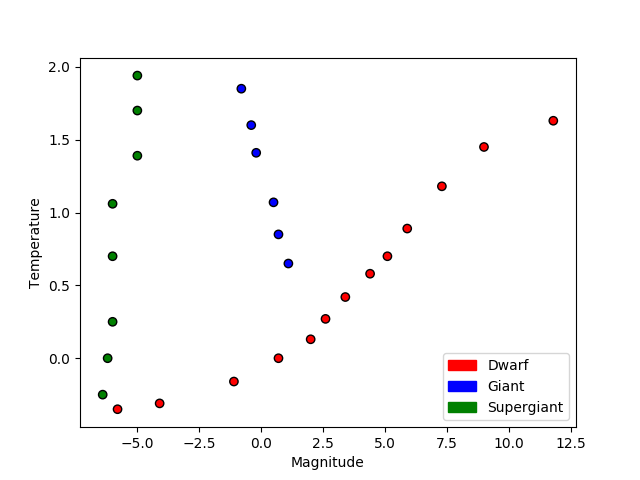
\includegraphics[width=0.8\textwidth]{star}
\caption{Magnitudes and temperatures of dwarf, giant, and supergiant stars. Adapted from \url{http://astrosci.scimuze.com/stellar_data.htm}}
\end{figure}
\begin{problem}[Classifying Stars, 15pts]
In this problem, you will code up two classifiers for this task:
\begin{itemize}
\item The three-class generalization of logistic regression, also
  known as softmax regression, for these data. You will do this by
  implementing gradient descent on the negative log likelihood. You
  will need to find good values for the learning rate $\eta$ and
  regularization strength $\lambda$. See the third practice problem in
  the section 3 notes for more information.
% FDV: Make sure the reference above is accurate
\item A generative classifier with Gaussian class-conditional
  densities, as in Problem~2. In particular, make two implementations:
  one with a shared covariance matrix across all of the classes, and
  one with a separate covariance being learned for each class.  (Note:
  the staff implementation can switch between these two with just a
  few lines of code.)
\end{itemize}
Implementation notes: you may use anything in \texttt{numpy} or
\texttt{scipy}, except for \texttt{scipy.optimize}.  The controller
file is \texttt{problem3.py}, in which you will specify
hyperparameters. The actual implementations you will write will be in
\texttt{LogisticRegression.py} and
\texttt{GaussianGenerativeModel.py}.  These files include class
interfaces for \texttt{GaussianGenerativeModel} and
\texttt{LogisticRegression}. The classes you implement follow the same pattern
as scikit-learn, so they should be familiar to you.  The code
currently outputs nonsense predictions just to show what the
high-level interface should be, so you should completely remove the
given \texttt{predict()} implementations and replace them with your
implementations.  You will also need to modify the hyperparameter
values.
\begin{enumerate}
\item Plot the decision boundaries with the \texttt{visualize()}
  function. Include these plots in your assignment PDF. What are the similarities and differences between the
  classifiers?  What explains the differences?
\item For logistic regression, plot negative log-likelihood loss with
  iterations on the x-axis and loss on the y-axis for several
  configurations of hyperparameters. Note which configuration yields
  the best final loss. Why are your final choices of learning rate
  ($\eta$) and regularization strength ($\lambda$) reasonable? How
  does altering these hyperparameters affect convergence? Focus both
  on the ability to converge and the rate at which it converges (a
  qualitative description is sufficient).
\item For both Gaussian generative models, report negative log
  likelihood. In the separate covariance matrix case, be sure to use
  the covariance matrix that matches the true class of each data
  point.
\item Finally, consider a star with magnitude 6 and temperature 2.
  To what class do each of the classifiers assign this star?  Do the
  classifiers give any indication as to whether or not you should
  trust them?
\end{enumerate}
\end{problem}
\subsection*{Solution}
\newpage
\begin{itemize}
    \item Name:
    \item Email:
    \item Collaborators:
    \item Approximately how long did this homework take you to complete (in hours):
\end{itemize}
\end{document}